% File:  /mit/8.13/presentations/zipped-sample-presentation/sample-presentation.tex
% Updated: June 11, 2008
% Summary: LaTeX template for creating Junior Lab presentations.
%
% Usage: To build a PDF, type `pdflatex sample-presentation.tex'
%        THREE TIMES in order to correct all internal references.
% The Beamer Package Users Guide can be viewed at
% /mit/8.13/presentations/beamerusersguide.pdf
% The users guide is a 224 page document so please don't print it out!

\documentclass[hyperref=pdftex, presentation]{beamer}
% Replacing 'presentation' with 'handout' in the above line
% will produce 4 slides per page.
% The hyperref option makes it possible to include hyperlinks.

\mode<presentation> {
  \usetheme{Boadilla}
  % or CambridgeUS, boxes, Warsaw, Madrid, many others
   %\setbeamercovered{transparent}
  % or whatever (possibly just delete it)
  }

\usepackage[english]{babel}
\usepackage[latin1]{inputenc}
\usepackage{times}
\usepackage[T1]{fontenc}
\usepackage{wrapfig}
\usepackage{graphicx}
\usepackage{adjustbox}
% Or whatever. Note that the encoding and the font should match. If T1
% does not look nice, try deleting the line with the fontenc.

\mode<handout>{
\usepackage{pgfpages}
\pgfpagesuselayout{4 on 1}[a4paper,landscape,border shrink=5mm]
\setbeamercolor{background canvas}{bg=black!10} }

%%%%%%%%%%%%%%%%%%%%%%%%%%%%%%%%%%%%%%%%%%%%%%%%%%%%%%%%%%%%%%%%%%%%%%

\title[Introduction to Magnetars] % (optional)
{Formation and Mechanics of High-Tesla Neutron Stars}

% \subtitle
% {Presentation Subtitle} % (optional)

\author[Gardner]{K.E.Gardner}
\institute[] {UTU - Department of Physics\\}
\date[\today]


% If you wish to uncover everything in a step-wise fashion, uncomment
% the following command:

% \beamerdefaultoverlayspecification{<+->}

% If you wish to uncover everything step by step step just add the command \pause on the specific place.
% Several places are suggested. Just uncomment \pause commands.
% Also- on Organization of talk  [pausesections] as an option.
% Adding the option [handout] to the \documentclass definition will automatically disable all \pause commands
% and will make the frame into slides- in nice printable format.

%;;;;;;;;;;;;;;;;;;;;;;;;;;;;;;;;;;;;;;;;;;;;;;;;;;;;;;;;;;;;;;;;;;;;;;;;;;;;;;;;;;;;;
\begin{document}
\begin{frame}
	\vspace*{-.5cm}
%	\begin{center}
%		\begin{figure}
%			\includegraphics[scale=.03]{UROP Logo.jpg}\hspace*{9cm}
%		\end{figure}
%	\end{center}
	%\vspace*{-1cm}
  \titlepage
\end{frame}




\begin{frame}{\Large What is a Magnetar?}
\frametitle{\Large What is a Magnetar?}

\begin{minipage}[0.2\textheight]{\textwidth}
\begin{columns}[T]
\begin{column}{0.5\textwidth}

\begin{block}{Definition:}

\begin{itemize}
 \item<2-> neutron star%\pause
 \item<3-> massive magnetic field ($\ge 10^{13}$ G)
\end{itemize}
\end{block}

\end{column}
\begin{column}{0.5\textwidth}
	\begin{figure}
		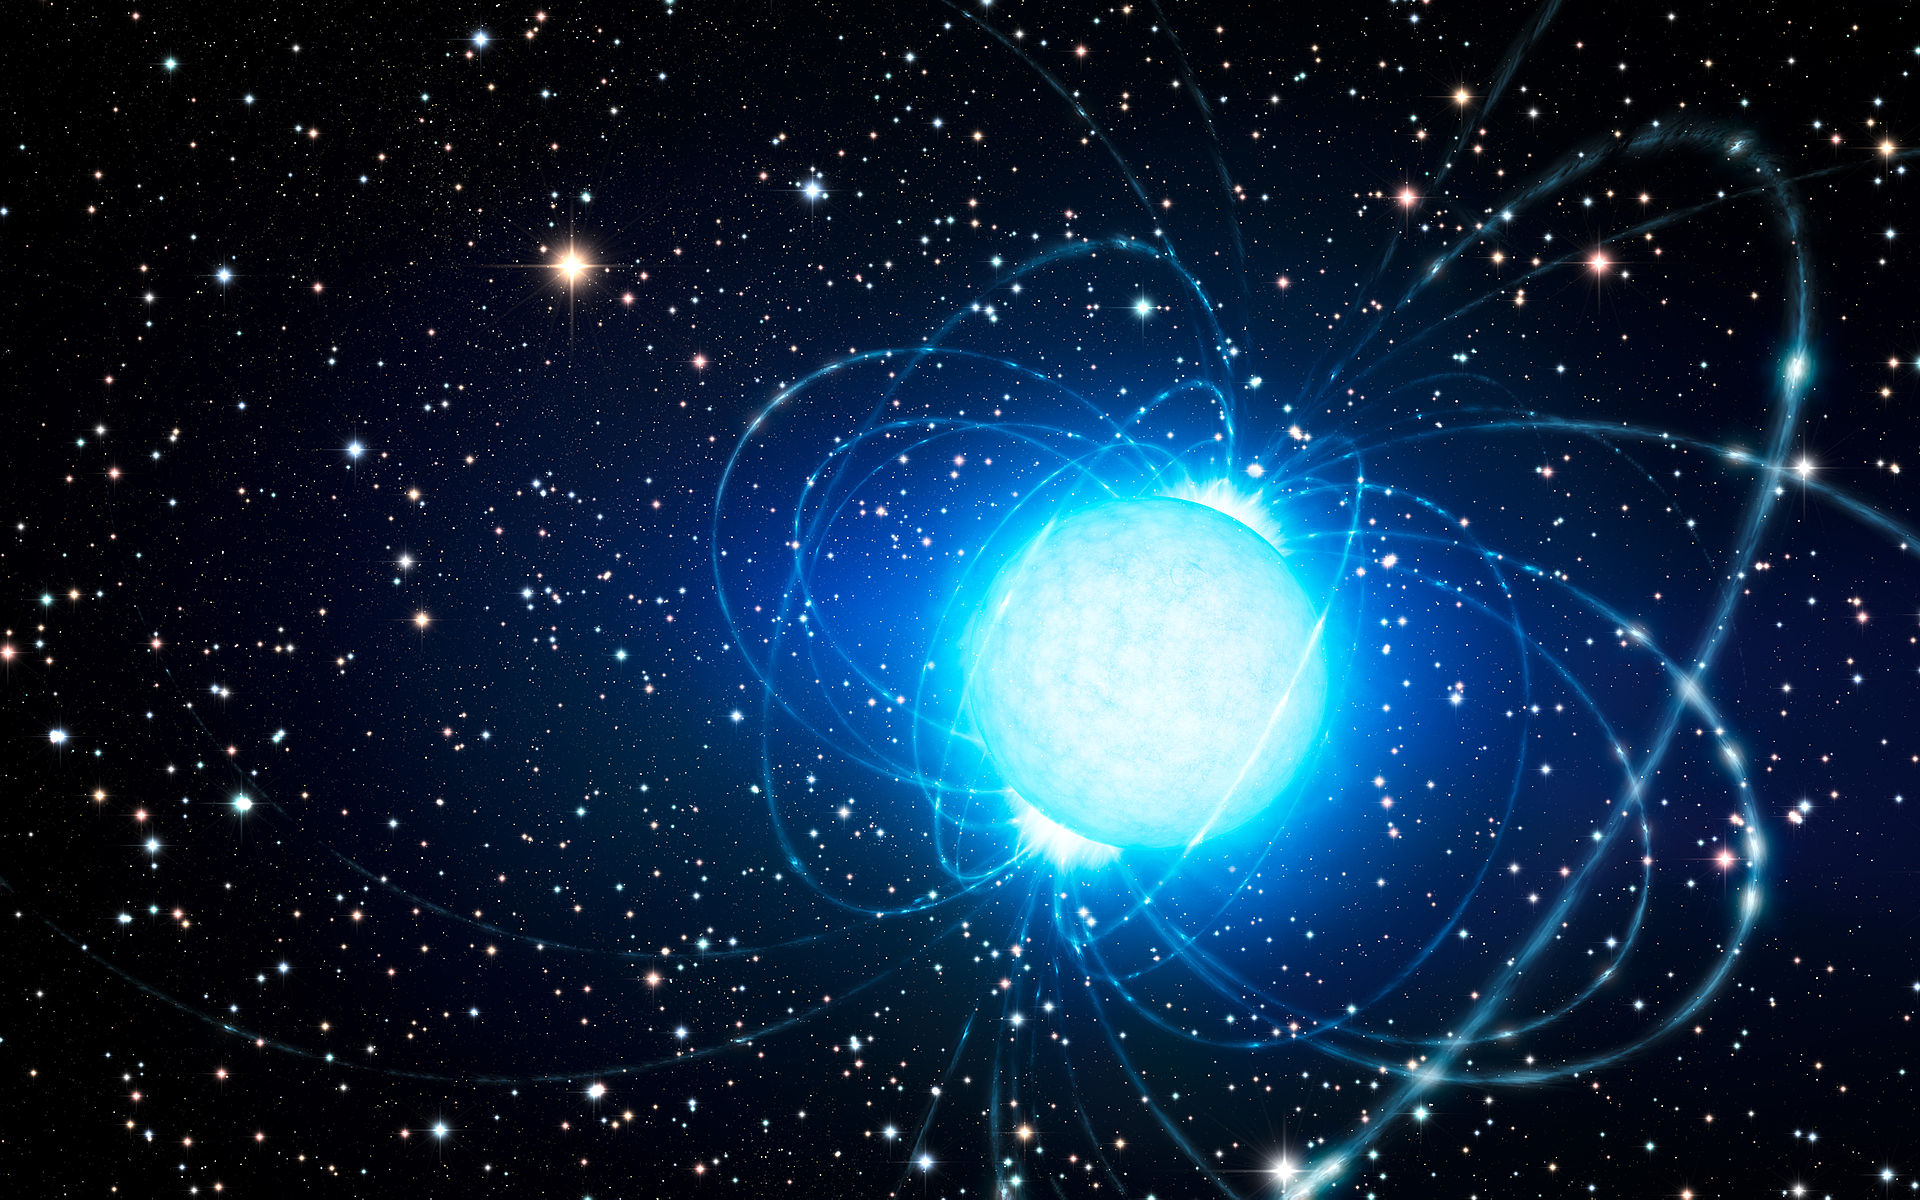
\includegraphics[scale=.09]{figures/magnetar_art.jpg}
		\caption{Artistic depiction of a magnetar}
	\end{figure}
\end{column}
\end{columns}
\end{minipage}

\end{frame}
%;;;;;;;;;;;;;;;;;;;;;;;;;;;;;;;;;;;;;;;;;;;;;;;;;;;;;;;;;;;;;;;;;;;;;;;;;;;;;;;;;;;;;

%columns & blocks: There are two handy environments for structuring
%your slide: "blocks", which divide your slide (horizontally) into
%headed sections, and "columns" which divides your slide (vertically)
%into colum%ns.  This next frame demonstrates both.

\begin{frame}{}
\frametitle{\Large Distinctions}
\begin{columns}[c] % the "c" option specifies center vertical
           % alignment, a `t' option would align the contents
           % top vertically

\column{.7\textwidth} % column designated by a command
\begin{block}{Detection}
\begin{itemize}
 \item<2-> 2-12s period X-Ray bursts%\pause
 \item<2-> large spin-down rates imply massive magnetic fields
\end{itemize}
\end{block}
\begin{block}{Sample}
\begin{itemize}
	\item<3-> Piezoelectric Suspension
	\item<3-> Indium-Tin Oxide coated PET plastic (0.01" thickness)
\end{itemize}
\end{block}
\column{.3\textwidth}


\end{columns}
\end{frame}




%;;;;;;;;;;;;;;;;;;;;;;;;;;;;;;;;;;;;;;;;;;;;;;;;;;;;;;;;;;;;;;;;;;;;;;;;;;;;;;;;;;;;;



%;;;;;;;;;;;;;;;;;;;;;;;;;;;;;;;;;;;;;;;;;;;;;;;;;;;;;;;;;;;;;;;;;;;;;;;;;;;;;;;;;;;;;


%columns & blocks: There are two handy environments for structuring
%your slide: "blocks", which divide your slide (horizontally) into
%headed sections, and "columns" which divides your slide (vertically)
%into colum%ns.  This next frame demonstrates both.
\begin{frame}{\Large Kinds of Magnetars}
	\begin{figure}
		\begin{columns}[c] % the "c" option specifies center vertical
           % alignment, a `t' option would align the contents
           % top vertically

			\column{.7\textwidth} % column designated by a command
			\begin{block}{Bi-modal}
				\begin{itemize}
					\item<1-> Persistent Magnetars
					\item<2-> Transient Magnetars
				\end{itemize}
			\end{block}
			\begin{block}{Cross-species}
				\begin{itemize}
 					\item<3-> Magnetar Pulsar%\pause
 					\item<4-> Theoretically: neutron star switch between magnetar, pulsar, and magnetar pulsar
				\end{itemize}
			\end{block}
			
			\column{.3\textwidth}

		\end{columns}
	\end{figure}
\end{frame}


\begin{frame}{\Large Budgeting}
	\begin{figure}
		\begin{columns}[c] % the "c" option specifies center vertical
           % alignment, a `t' option would align the contents
           % top vertically
			
			\column{.7\textwidth} % column designated by a command
			\begin{block}{Materials}
				\begin{itemize}
 					\item<2-> BaTiO3 nanoparticles - \$30/25g%\pause
 					\item<3-> Flexible Photopolymer - \$90/1kg
 					\item<4-> Indium Tin Oxide PET - \$5/(32 sq.in. sheet)
				\end{itemize}
			\end{block}
			\begin{block}{Per Sample}
				\begin{itemize}
 					\item<2-> 0.04g BaTiO3 nanoparticles
 					\item<3-> .2g Flexible Photopolymer
 					\item<4-> 1.5 sq.in. Indium Tin Oxide PET
				\end{itemize}
			\end{block}
			\begin{itemize}
				\item<5-> Total Cost per sample: \$0.30
			\end{itemize}
			
			\column{.3\textwidth}
		\end{columns}
	\end{figure}
\end{frame}


\begin{frame}{\Large Standards}
	\begin{figure}
		\begin{columns}[c] % the "c" option specifies center vertical
           % alignment, a `t' option would align the contents
           % top vertically
			
			\column{.7\textwidth} % column designated by a command
			\begin{itemize}
				\item 176-1987 - IEEE Standard on Piezoelectricity (withdrawn)
				\item No other applicable standards were found
			\end{itemize}
			
			\column{.3\textwidth}
		\end{columns}
	\end{figure}
\end{frame}


%;;;;;;;;;;;;;;;;;;;;;;;;;;;;;;;;;;;;;;;;;;;;;;;;;;;;;;;;;;;;;;;;;;;;;;;;;;;;;;;;;;;;;
\begin{frame}{Typical Response (Plucking)}
 \begin{block}{Control Test:}
 \begin{center}
%\begin{figure}
%	\includegraphics[scale=.25]{cresp1.png}
%\end{figure}
 \end{center}
\end{block}
\end{frame}



%;;;;;;;;;;;;;;;;;;;;;;;;;;;;;;;;;;;;;;;;;;;;;;;;;;;;;;;;;;;;;;;;;;;;;;;;;;;;;;;;;;;;;
\begin{frame}{Typical Response (Plucking)}
 \begin{block}{6 wt\% Test:}
 \begin{center}
%\begin{figure}
%	\includegraphics[scale=.25]{6resp1.png}
%\end{figure}
 \end{center}
  \end{block}
\end{frame}


%;;;;;;;;;;;;;;;;;;;;;;;;;;;;;;;;;;;;;;;;;;;;;;;;;;;;;;;;;;;;;;;;;;;;;;;;;;;;;;;;;;;;;
\begin{frame}{Typical Response (Plucking)}
 \begin{block}{11 wt\% Test:}
 \begin{center}
%\begin{figure}
%	\includegraphics[scale=.25]{11resp2.png}
%\end{figure}
 \end{center}
  \end{block}
\end{frame}


%;;;;;;;;;;;;;;;;;;;;;;;;;;;;;;;;;;;;;;;;;;;;;;;;;;;;;;;;;;;;;;;;;;;;;;;;;;;;;;;;;;;;;
\begin{frame}{Typical Response (Plucking)}
 \begin{block}{20 wt\% Test:}
 \begin{center}
%\begin{figure}
%	\includegraphics[scale=.25]{20resp1.png}
%\end{figure}
 \end{center}
 \end{block}
\end{frame}


%;;;;;;;;;;;;;;;;;;;;;;;;;;;;;;;;;;;;;;;;;;;;;;;;;;;;;;;;;;;;;;;;;;;;;;;;;;;;;;;;;;;;;
\begin{frame}{Sources of Uncertainty}
\begin{center}
\end{center}
\begin{itemize}
\item Force measurement
\item Unknown polymer structure
\item Noisy Environment
\end{itemize}
\end{frame}

%;;;;;;;;;;;;;;;;;;;;;;;;;;;;;;;;;;;;;;;;;;;;;;;;;;;;;;;;;;;;;;;;;;;;;;;;;;;;;;;;;;;;;



%;;;;;;;;;;;;;;;;;;;;;;;;;;;;;;;;;;;;;;;;;;;;;;;;;;;;;;;;;;;;;;;;;;;;;;;;;;;;;;;;;;;;;
\begin{frame}{Summary and Conclusions}

  % Keep the summary *very short*.
  \begin{columns}[c] % the "c" option specifies center vertical
           % alignment, a `t' option would align the contents
           % top vertically

			\column{.7\textwidth} % column designated by a command
			\begin{block}{Successes}
				\begin{itemize}
 					\item<2-> The new material is piezoelectric %
					\item<3-> Samples exhibit significant electrical responses.
					\item<4-> Sample construction is cheap and accessible
				\end{itemize}
			\end{block}
			\begin{block}{Further Study}
				\begin{itemize}
 					\item<5-> Better understand the polymer %
					\item<6-> Explore other piezoelectric ceramic nanoparticles.
					\item<7-> Determine how to use suspension in 3D printing.
				\end{itemize}
			\end{block}
			\column{.3\textwidth}

		\end{columns}
\end{frame}


\begin{frame}{Resources}
	\begin{itemize}
		\item Project Files: https://github.com/mflibby/FlexPiezo
		\item Samples Request: mackenzieflibby@gmail.com
	\end{itemize}
\end{frame}

\begin{frame}{References}
	\begin{itemize}
		\item Cui, H., Hensleigh, R., Yao, D., Maurya, D., Kumar, P., Kang, M. G., Zheng, X. (R. (2019). Three-dimensional printing of piezoelectric materials with designed anisotropy and directional response. Nature Materials, 18(3), 234-241. doi: 10.1038/s41563-018-0268-1
		\item Fu, J., Hou, Y., Zheng, M., \& Zhu, M. (2020). Flexible Piezoelectric Energy Harvester with Extremely High Power Generation Capability by Sandwich Structure Design Strategy. ACS Applied Materials \& Interfaces, 12(8), 9766-9774. doi: 10.1021/acsami.9b21201
		\item Yang, Y., Pan, H., Xie, G., Jiang, Y., Chen, C., Su, Y.,  Tai, H. (2020). Flexible piezoelectric pressure sensor based on polydopamine-modified BaTiO3/PVDF composite film for human motion monitoring. Sensors and Actuators A: Physical, 301, 111789. doi: 10.1016/j.sna.2019.111789
	\end{itemize}
\end{frame}

\end{document}
